\documentclass[a4paper, 10pt, twoside, openright]{book}
\usepackage[T1]{fontenc}
\usepackage{times}
\usepackage{graphicx}
\usepackage[usenames,dvipsnames]{color}
\usepackage{fancyhdr}
\usepackage{sectsty}
\usepackage{listings}
\usepackage{float}
\usepackage[fit]{truncate}
\usepackage{amsmath}
\usepackage{multirow}
\usepackage{pdfpages}
\usepackage{tikz}
\usepackage[fancy,color=orange]{tikz-inet}
\usepackage{amssymb}
\usepackage{booktabs}


% Bibliography setting and style
\usepackage[backend=bibtex8,mincrossrefs=99,style=alphabetic,doi=false,isbn=false,url=false,refsegment=chapter,defernumbers=true,sorting=nyt]{biblatex}
\addbibresource{Thesis.bib}
\defbibheading{subbibliography}{\addcontentsline{toc}{section}{References}\section*{References}}

\newcommand{\dataflow}{data-flow}
\newcommand{\Dataflow}{Data-flow}
\newcommand{\code}[1]{\texttt{\lstinline[basicstyle=\normalsize\ttfamily,identifierstyle={\normalsize},commentstyle={\normalsize\itshape},keywordstyle={\normalsize\bfseries},ndkeywordstyle={\normalsize},stringstyle={\normalsize\ttfamily},numberstyle={\normalsize}]!#1!}}
\newcommand{\CFG}{CFG}
\newcommand{\intraj}{\textsc{Intra}J}
\newcommand{\jastaddjintraflow}{\textsc{jastaddj-intraflow}}
\newcommand{\jji}{\code{JJI}}
\newcommand{\cG}{\mathcal{G}}
\newcommand{\cV}{\mathcal{V}}
\newcommand{\cE}{\rightarrowtail}
\newcommand{\cP}{\mathcal{P}}
\newcommand{\cM}{\mathcal{M}}

\newcommand{\mSyn}{\ensuremath{\uparrow}}
\newcommand{\mInh}{\ensuremath{\downarrow}}
\newcommand{\mHOA}{\ensuremath{\rightarrow}}
\newcommand{\mColl}{\ensuremath{\square}}
\newcommand{\mCirc}{\ensuremath{\circlearrowleft}}

\newcommand{\Abase}[1]{\textcolor{ATGsym}{\mbox{\umlcode{#1}}}}
\newcommand{\Asyn}[2]{\textcolor{ATGsym}{\mbox{\umlcode{\astnode{#1}}.\mSyn{}\umlcode{#2}}}}
\newcommand{\Asynaccess}[2]{\umlcode{get}\textcolor{ATGsym}{\mbox{\umlcode{\astnode{#1}}\textcolor{black}{\umlcode{()}}.\mSyn{}\umlcode{#2}\textcolor{black}{()}}}}
\newcommand{\Ainh}[2]{\textcolor{ATGsym}{\mbox{\umlcode{\astnode{#1}}.\mInh{}\umlcode{#2}}}}
\newcommand{\Ainhdef}[3]{\textcolor{ATGsym}{\mbox{\umlcode{\astnode{#1}}.\umlcode{\astnode{#2}}.\mInh{}\umlcode{#3}}}}
\newcommand{\Ahoa}[2]{\textcolor{ATGsym}{\mbox{\umlcode{\astnode{#1}}.\mHOA{}\umlcode{#2}}}}
\newcommand{\Acoll}[2]{\textcolor{ATGsym}{\mbox{\umlcode{\astnode{#1}}.\mColl{}\umlcode{#2}}}}

\newcommand{\AcircSyn}[2]{\textcolor{ATGsym}{\mbox{\umlcode{\astnode{#1}}.\mSyn{}\umlcode{#2}\mCirc{}}}}



\newcommand{\umlcode}[1]{\textrm{#1}}  % Style of code used in UML fragments
\newcommand{\astnodestyle}{\ttfamily\color{magenta}}
\newcommand{\astnode}[1]{\texttt{\textcolor{magenta}{#1}}}  % Style used for AST node types

\newcommand{\ASTUnrestricted}{AST-unrestricted}
\newcommand{\ParentFirst}{Parent-First}

\newcommand{\project}[1]{\textsc{#1}}
\newcommand{\tool}[1]{\textsc{#1}}

% can't get fbox to work reliably in the UML code, and adjustbox and nested \tikz don't work at all
%\newcommand{\dfapi}{\textsf{\setlength{\fboxsep}{0pt}\fcolorbox{blue}{white}{df-api}}}
\newcommand{\dfapi}{\textbf{\textcolor{black}{[df-api]}}}
\newcommand{\nameapi}{\textbf{\textcolor{black}{[name-api]}}}

\newcommand{\frameworkname}{\textsc{Intra}CFG}
\newcommand{\intracfg}{\textsc{\frameworkname}}

\newcommand{\node}{\mathsf{n}}
\newcommand{\Null}{\mathtt{NULL}}
\newcommand{\Notnull}{\mathtt{NOTNULL}}
\newcommand{\gen}{\mathtt{gen}}
\renewcommand{\kill}{\mathtt{kill}}

\newcommand{\In}{\mathtt{in}}
\newcommand{\Out}{\mathtt{out}}
\newcommand{\Use}{\mathtt{use}}
\newcommand{\Def}{\mathtt{def}}
\newcommand{\tf}{f_t}
\newcommand{\mCi}[1]{ { \textcolor{black!30}{\scriptstyle \pm\text{#1}}}}%Condifdence interval

\newcommand{\CR}[1]{\textbf{[}\textcolor{blue!60!black}{\textbf{CR:} #1}\textbf{]}}
\newcommand{\Ckw}[1]{\texttt{\textbf{#1}}}
\newcommand{\auxlabel}[1]{{\scriptsize{$\textrm{\texttt{#1}}$}}}
\newcommand{\auxlabeli}[2]{{\scriptsize{$\textrm{\texttt{#2}}_{#1}$}}}
\newcommand{\auxlabelbox}[1]{\tikz[baseline=-0.7ex] \node[rectangle, minimum width=0, thin, draw, rounded corners, fill=white, inner sep=2pt, outer sep=0pt] (N) {\auxlabel{#1}};}
\newcommand{\auxlabelboxhoa}[1]{\tikz[baseline=-0.7ex] \node[rectangle, dashed,minimum width=0, thin, draw, rounded corners, fill=white, inner sep=2pt, outer sep=0pt] (N) {\auxlabel{#1}};}

%\newcommand{\auxlabelboxi}[2]{\tikz \node[rectangle, minimum width=0, thin, draw, rounded corners, fill=white] {\auxlabeli{#1}{#2}};}


\newcommand{\Prod}{::=}
\newcommand{\terminal}[1]{\textcolor{green!50!black}{\textit{#1}}}
\newcommand{\vmetavar}[1]{\textcolor{cyan!30!black}{\textsf{\textbf{#1}}}}
\newcommand{\vcode}[1]{\textsf{\textcolor{green!35!black}{{#1}}}}
\newcommand{\vterminal}[1]{\vcode{#1}}
\newcommand{\nta}[1]{\ensuremath{\textit{#1}}}
\newcommand{\tuple}[1]{\ensuremath{\langle #1 \rangle}}
\newcommand{\nt}[1]{\ensuremath{\tuple{\hspace{-0.02cm}\nta{#1}\hspace{0.02cm}}}}
\newcommand{\VB}{\ |\ }
\newcommand{\Gcomment}[1]{\textrm{\textcolor{black!50!white}{({#1})}}}
\newcommand{\sem}[1]{\ensuremath{\llbracket #1 \rrbracket}}
%\newcommand{\semNPA}[1]{\ensuremath{\sem{#1}_{\textit{NPA}}}}
\newcommand{\semNPA}[1]{\ensuremath{\sem{#1}}}

\newcommand{\listingsfontsize}{\scriptsize}

\newcommand{\NAmark}{\multicolumn{1}{c}{\textcolor{black!40!white}{-}}}
\newcommand{\NAmarkR}{\multicolumn{1}{c|}{\textcolor{black!40!white}{-}}}
\newcommand{\Tcenter}[1]{\multicolumn{1}{c}{#1}}
\newcommand{\TcenterR}[1]{\multicolumn{1}{c|}{#1}}
\newcommand{\succarrow}{\tikz[baseline=-0.7ex] \draw[succarrow, thick, -{Stealth[scale=0.9, inset=0pt, angle'=45]}] (0,0) -- (0.3,0.0);}

\colorlet{hlgreen}{green}
\colorlet{hlorange}{orange}
\colorlet{hlgreenhalf}{green!50!white}
\colorlet{hlorangehalf}{orange!50!white}

\DeclareRobustCommand{\hlgreen}[1]{{\sethlcolor{hlgreenhalf}\hl{#1}}}
\DeclareRobustCommand{\hlorange}[1]{{\sethlcolor{hlorangehalf}\hl{#1}}}

\definecolor{ATGsym}{HTML}{206010}

\definecolor{SQ}{HTML}{0080ff}
\definecolor{JJI}{HTML}{ff0080}
\definecolor{IJnonH}{HTML}{004010}
\definecolor{IJH}{HTML}{00ff20}

\definecolor{succarrow}{HTML}{4e90e2}	% adapted from RunningExample.tex

\definecolor{lightblue}{HTML}{006699}		%#006699
\definecolor{lightgreen}{HTML}{669900}		%#669900
\lstdefinelanguage{JastAdd}{
  %keyword1&2&6
  morekeywords = [1]{aspect, abstract, class, continue, default, enum, extends, false, final, finally, implements, import, instanceof, interface, native, new, null, package, private, protected, public, static, strictfp, throws, transient, true, void, volatile, length, assert, case, return, super, this, throw, catch, do, if, else, switch, synchronized, while, try, ?},
  %keyword3
  morekeywords = [2]{inh, syn, coll, with, eq, NTA, contributes, to, for, each, circular, with}, %JASTADD keywords
  %keyword4
  morekeywords = [3]{CFGNode, Assignments, Assign,AssignBitwiseExpr, TrueLiteral, Entry,ConstructorDecl,UnceckedException, TryWithResorucesStmt, NTAFinallyBlock,ClassDecl, CloseListNTA, BreakStmt,ThrowStmt,TryStmt,ReturnStmt, ContinueStmt, Exit, Expr, AssignShiftExpr, AssignMultiplicativeExpr, IntegerLiteral, AssignAdditiveExpr, UnaryIncDec,DoStmt,VariableDeclarator, NumericLiteral, ParameterDeclaration, FieldDeclarator, PostfixExpr, PreIncExpr, PreDecExpr, ReachedLVal, Variable,EQOp,CFGSupport, ForStmt, EmptyStmt, MethodDecl, ExprStmt, AssignStmt, IfStmt, AndOp, LessOp, WhileStmt, Block, AssignExpr, PostUnaryInc, PostUnaryDec, Entry, Exit, EQExpr, VarAccess, CFGRoot }, %ASTnode typess
  %keyword5
  morekeywords = [4]{Array, ArrayList, Boolean, Byte,  BitSet, BufferedReader,Collections, Character, Class, Double, Float, Gamma, AbsDomain, NULL, NOTNULL, TOP,Integer, HashMap, PrintWriter, String, StringBuffer, StringBuilder, Thread, boolean, byte, char, color, double, float, int,Type, long, short, FloatDict, FloatList, IntDict, IntList, JSONArray, JSONObject, PFont, PGraphics, PImage, PShader, PShape, PVector, StringDict, StringList, Table, TableRow, XML, Set, HashSet},
  %keywordstyle = [1]\color{lightblue},
  %keywordstyle = [2]\color{lightgreen},
  keywordstyle = [1]\bfseries,
  keywordstyle = [2]\bfseries,
  keywordstyle = [3]\astnodestyle,
  keywordstyle = [4]\color{orange},
  sensitive = true,
  morecomment = [l]{//},
  morecomment = [s]{/*}{*/},
  morecomment = [s]{/**}{*/},
  commentstyle = \color{gray},
  morestring = [b]",
  morestring = [b]',
  stringstyle = \color{purple},
  frame=none
}
\lstset{
  basicstyle=\listingsfontsize\ttfamily,
  identifierstyle={\listingsfontsize},
  commentstyle={\listingsfontsize\itshape},
  keywordstyle={\listingsfontsize\bfseries},
  ndkeywordstyle={\listingsfontsize},
  stringstyle={\listingsfontsize\ttfamily},
  frame={tb},
  breaklines=true,
  breakatwhitespace=true, %To avoid linebreaks between \code{} and comma.
  columns=[l]{fullflexible},
  numbers=none,
  numberstyle={\listingsfontsize},
  stepnumber=1,
  mathescape
%	escapeinside     = {@}{@}, %General escape does not seem to work in lstinline/GH.
}

\makeatletter
\pgfdeclareshape{topbottombox}{
  \inheritsavedanchors[from=rectangle]
  \inheritanchorborder[from=rectangle]
  \inheritanchor[from=rectangle]{center}
  \inheritanchor[from=rectangle]{base}
  \inheritanchor[from=rectangle]{north}
  \inheritanchor[from=rectangle]{north east}
  \inheritanchor[from=rectangle]{east}
  \inheritanchor[from=rectangle]{south east}
  \inheritanchor[from=rectangle]{south}
  \inheritanchor[from=rectangle]{south west}
  \inheritanchor[from=rectangle]{west}
  \inheritanchor[from=rectangle]{north west}
  \backgroundpath{
    %  store lower right in xa/ya and upper right in xb/yb
    \southwest \pgf@xa=\pgf@x \pgf@ya=\pgf@y
    \northeast \pgf@xb=\pgf@x \pgf@yb=\pgf@y
    \pgfpathmoveto{\pgfpoint{\pgf@xa}{\pgf@ya}}
    \pgfpathlineto{\pgfpoint{\pgf@xb}{\pgf@ya}}
    \pgfpathmoveto{\pgfpoint{\pgf@xa}{\pgf@yb}}
    \pgfpathlineto{\pgfpoint{\pgf@xb}{\pgf@yb}}
 }
}
\makeatother


% Patch UML package pgf-umlcd to be able to write abstract grammar as class name.

\newbool{ANON}
%\booltrue{ANON}
\boolfalse{ANON}
\newcommand{\anon}[2]
{\ifbool{ANON}{
   #1
}{
   #2
}}


\defbibheading{bibintoc}{%
 \addcontentsline{toc}{chapter}{\bibname}%
 \section*{References}}


\begin{document}

\frontmatter

%------------------------------------
% title page
%------------------------------------
\begin{titlepage}

\thispagestyle{empty}
\includepdf[pages=-,offset=16mm 0mm]{frontpage.pdf}

\begin{flushleft}
\vspace*{\stretch{1}}

%\Large \textbf{NB! Draft created on \today} \normalsize\\[2cm]

ISBN (eletronic version) TODO\\
ISBN (print version) TODO\\
ISSN TODO\\
Dissertation TODO\\
LU-CS-DISS:2012-4\linebreak[2]

Department of Computer Science \\
Lund University \\
Box 118 \\
SE-221 00  Lund \\
Sweden  \linebreak[2]

Email: \url{idriss.riouak@cs.lth.se} \linebreak[2]

Typeset using \LaTeX \\

Printed in Sweden by Tryckeriet i E-huset, Lund, 2022\linebreak[2]

\textit{\copyright ~2022 Idriss Riouak}
\vspace{10mm}
\end{flushleft}
\end{titlepage}
%------------------------------------






%------------------------------------
% kappa
%------------------------------------

\chapter{Abstract}


Static program analysis plays a crucial role in ensuring the quality and security of
software applications by detecting and fixing bugs,
and potential security vulnerabilities in the code. The utilization of declarative paradigms
in dataflow analysis as part of this process has become increasingly popular in recent years.\\[5pt]

The aim of this thesis is to explore the design and implementation of \emph{control-flow} and 
\emph{dataflow} analyses using the \emph{Reference Attribute Grammars} formalism.
Specifically, we focus on the construction of analyses directly on the source code
rather than on an intermediate representation.\\[5pt]

The main result, summarised in this thesis, is our language-agnostic framework, called \textsc{IntraCFG}.
\textsc{IntraCFG} enables efficient and effective dataflow analysis by allowing the construction of precise and
lightweight source-level control-flow graphs. The framework superimposes control-flow
graphs on top of the abstract syntax tree of the program. The effectiveness of the \textsc{IntraCFG} framework is
demonstrated through two case studies, \textsc{IntraJ} and \textsc{IntraTeal}, that
show the potential and the flexibility of \textsc{IntraCFG} in different contexts,
such as, bug detection and teaching.
\textsc{IntraJ}, has proven to be faster and precise as well-known
industrial tools. Its precision and performance, combined with
on-demand evaluation, make \textsc{IntraJ} an ideal tool for use in
Integrated Development Environments.
Additionally, this thesis presents \textsc{JFeature}, a tool for automatically extracting
and summarising the key features of a corpus of Java programs. \textsc{JFeature} allows
researcher and developers to gain a deeper understanding of the characteristics of a codebase and
can be used to evaluate the effectiveness of their tools and techniques.

\section{\textsc{IntraCFG}: Intraprocedural Framework for Source-Level Control-Flow Analysis}%
\label{sec:IntraCFG}
The techniques of CFGs construction has seen significant advancements
in recent years, with various frameworks being proposed to aid in the construction
of precise intraprocedural CFGs~\cite{smits2020flowspec,10.1016/j.scico.2012.02.002}.
We contribute to the state-of-the-art by introducing \textsc{IntraCFG}, a declarative, RAG-based,
and language-independent framework for constructing precise intraprocedural CFGs.

Unlike most other frameworks, which build CFGs on the IR level,
e.g.,  bytecode, \textsc{IntraCFG}'s approach superimposes the CFGs
on the AST. This allows for a more accurate client analysis,
as the CFGs are constructed directly on the source code level, rather than an
intermediate representation. Additionally, this approach also enables the construction
of \textsc{AST-Unrestricted} CFGs, which are CFGs whose shape is not restricted to the AST structure.
\subsection{Overall Architecture}
The overall architecture of our proposed framework, \textsc{IntraCFG}, and its
ecosystem\todo{Not sure about the word ecosystem} is shown in Figure~\ref{fig:intraCFG}.
The framework provides the skeleton and default behaviour for construction of CFGs,
which can be instantiated for specific languages\footnote{\textbf{\texttt{IntraX}} in the diagram.}, e.g., Java or Teal.
\begin{figure}[H]
    \centering
    \includegraphics[width=1\textwidth]{kappa/img/architecture.pdf}
    \caption{\label{fig:intraCFG} Overall architecture of \textsc{IntraCFG} and its ecosystem.}
\end{figure}

The framework consists of several key components, including interfaces
(e.g., \textsc{CFGRoot}, \textsc{CFGSupport}, and \textsc{CFGNode}), attribute equations that define the
default behavior, and user APIs. The interfaces provide the structure for the
CFG and the attribute equations define the default behavior for the CFG
construction. Language specific AST nodes implement the different interfaces
according to the level of precision desired for the CFG.
The framework expose the CFG to the client analysis through APIs, that can be used
to query the CFG for information, such as the entry and exit nodes, or to traverse the CFG.
The language-independent nature of \textsc{IntraCFG} allows for easy integration
with various programming languages and enables the construction of precise CFGs
for those languages. The use of attribute equations and interfaces also allows
for a high degree of flexibility in the CFG construction process,
enabling the customization of the CFG to fit the specific needs of the
analysis being performed.

% Additionally, language-specific dataflow analysis, such as \texttt{NullPointerException} or
% \texttt{IndexOutOfBound} detection, can be built on top of the framework.





\subsection{\textsc{IntraCFG} for Java}
To demonstrate \textsc{IntraCFG} applicability, we developed
\textsc{IntraJ}, an instance of the framework for the Java programming language.
We built \textsc{IntraJ} as an extension of the \textsc{ExtendJ} extensible Java compiler~\cite{DBLP:conf/oopsla/EkmanH07}.
The complete architecture of \textsc{IntraJ} is shown in Figure~\ref{fig:intraJ}.
\begin{figure}[H]
    \centering
    \includegraphics[scale=0.52]{kappa/img/architecturejava.pdf}
    \caption{\label{fig:intraJ} Overall architecture of \textsc{IntraCFG} instansiated for the Java language.}
\end{figure}

%Discussing modularity
We designed \textsc{IntraJ}, following a  modular approach, and we separately
instansiated the framework for different versions of Java such as Java 4,
Java 5, Java 7 and Java 8. Each version of Java is implemented as a separate
aspect of the compiler. This approach allows us and the users of \textsc{IntraJ}
to easily extend the framework to support new versions of Java.

% Discussing precision
The degree of precision in creating CFGs using \textsc{IntraCFG} can differ in order
to meet the requirements of a given application.
This flexibility allows us to optimize the efficiency of the analysis by selectively
excluding certain nodes from the CFG, such as \texttt{WhileStmt}, which do not
provide any information relevant to the analyses.
\begin{figure}[H]
	\centering
	\begin{tikzpicture}
		\node (a) at (3.5,0) {\includegraphics[scale=0.55]{kappa/img/exampleAST.pdf}};
		\node[scale=0.65] (b) at (-0.6,0.7) {
			\begin{lstlisting}[language=JastAdd]
void foo(boolean b){
  String x = null;
  if(b) {
    x = "Hello World";
  }
  x.toString();
}
			\end{lstlisting}
		};
	\end{tikzpicture}
	\caption{\label{fig:CFG} CFG of the \texttt{foo} Java method.}
\end{figure}

The example in Figure~\ref{fig:CFG} is a visual representation of the AST and CFG of the
\texttt{foo} Java method. The figure illustrates the ability of the framework to tailor the CFG
to the specific requirements of the analysis and eliminate unnecessary complexity for improved performance.
In this example, nodes like \texttt{IfStmt} or \texttt{Dot} are not included in the CFG,
resulting in a more concise but precise representation of the control flow of the program.
On the other hand, the precision of the CFGs can be improved by synthethizing new nodes and new subtrees.
For instance, we designed \textsc{IntraJ} to compute an exception-sensitive
control-flow analysis, i.e., new AST subtrees are synthesized for each possible exceptional path.
The resulting CFGs are more precise, but they are also more complex, resulting
in a higher memory consumption and a longer analysis time.



In \textsc{IntraJ}, we implemented five different dataflow analyses:
\begin{itemize}
  \item \emph{Live Variable Analysis}: This analysis computes the set of variables that are live at each program point.
  \item \emph{Reaching Definition}: computes the set of definitions that reach each program point.
  \item \emph{Null Pointer Analysis}: detects possible null pointer dereferences.
  \item \emph{Dead Assignment Analysis}: detects assignments to l-values that are never used from that point on.
  \item \emph{Indirect Dead Assignment Analysis}: detects assignments to l-values which uses always flow to a dead assignment.
\end{itemize}
All the analyses relie on the result of the control-flow analysis. To the analysis are exposed
the entry and exit nodes of the CFG, as well as the successor and predecessor
nodes of each node.
Each analysis is implemented as a separate aspect of the compiler. Nevertheless,
the result of some analyses is used as input for other analyses. For instance,
the result of Live Variable Analysis is used as input for the Dead Assignment Analysis.
Similarly, the result of Dead Assignment Analysis is used to compute Indirect Dead Assignment Analysis.

The implemented analyses are instances of the monotone frameworks (see Section~\ref{sec:monotoneframeworks}).
Each analysis defines its abstract domain, transfer function and \emph{in} and
\emph{out}\footnote{Sometimes can be named \emph{gen} and \emph{kill}.} attributes.
The language dependency of the dataflow analysis arises from the fact that the
transfer function, which defines the relationship between the \emph{in} and \emph{out},
is modeled as an attribute. This transfer function attribute is
define for each AST node in the CFG in order to capture the semantic of passing
through that node.


\subsubsection{\textsc{IntraJ} Artifact Evaluation}
Artifact evaluation is an important part of the scientific process as it enables 
researchers to demonstrate the reproducibility and practicality of their work. 
It also allows other researchers to build upon and reuse the work in their own 
studies, helping to advance the field as a whole.

In this context, our artifact, \textsc{IntraJ}, was presented at the 
ROSE\footnote{\textbf{R}ecognizing and Rewarding \textbf{O}pen Science in \textbf{SE}, 
\url{https://icsme2021.github.io/cfp/AEandROSETrack.html}} Festival 2021, 
co-located with ICSME2021 and SCAM2021. The artifact was awarded the \emph{Open Research Objects} 
(ORO) and \emph{Research Objects Reviewed} (ROR) badges, which demonstrate its high level of documentation 
and structure, making it easily accessible and reusable by other researchers.
\begin{figure}[htbp]
  \centering
  \begin{subfigure}{0.3\linewidth}
    \includegraphics[width=\linewidth]{kappa/img/Open_research.png}
    \caption{Open Research Objects (ORO) badge}
    \label{fig:ORO}
  \end{subfigure}\hspace{2cm}
  \begin{subfigure}{0.3\linewidth}
    \includegraphics[width=\linewidth]{kappa/img/Research_Objects.png}
    \caption{Research Objects Reviewed (ROR) badge}
    \label{fig:ROR}
  \end{subfigure}
  \caption{Badges awarded to the artifact.}
  \label{fig:badges}
\end{figure}

Our artifact was well documented, with a clear and concise README.md, and was easy to 
use, with a self-contained script that enabled reviewers to easily reproduce the 
results presented in our paper. These factors helped to demonstrate the practicality 
and reliability of our work, and allowed other researchers to build upon our findings.


\subsection{\textsc{IntraCFG} for TEAL}
\begin{figure}[H]
    \centering
    \includegraphics[scale=0.65]{kappa/img/architectureteal.pdf}
    \caption{\label{fig:IntraTeal} Overall architecture of \textsc{IntraCFG} instansiated for the Teal language.}
\end{figure}
As a further demonstration of the applicability of \textsc{IntraCFG},
we developed \textsc{IntraTeal}, an implementation of the framework for the Teal programming language.
The teal programming language is used for teaching purposes
and provides a simple and easy-to-learn syntax for students to understand the
concepts of static program analysis (see Section~\ref{sec:teal}).
As part of the course, the complete source code of \textsc{IntraTeal} was provided to students along with
instructions and guidelines for utilizing the API to implement their own analyses.
We also made available a reference implementation of the
\texttt{NullPointerException} analysis. We then asked students, as a way of
extending their understanding and skills, to implement an \texttt{IndexOutOfBound}
analysis on the interval abstract domain. This exercise provided the
students with an opportunity to apply the concepts they had learned in a practical
setting and gain a deeper understanding of dataflow analysis.

Another key aspect of both, \textsc{IntraTeal} and \textsc{IntraJ} implementations, is that they
construct enhanced control-sensitive CFGs. Control-sensitive CFGs
are a more precise representation of the control flow of a program, as they take
into account the specific control flow behavior of a program. This is achieved by
synthesizing two AST nodes, i.e., \texttt{ControlTrue} and \texttt{ControlFalse} for each
comparison operator, e.g.,  ``$\le$'', ``$==$'', ``$!=$'', inside a conditional statement.
These HOAs are used to represent the control flow of the program and the information that ca be inferred from
it. \\
%
\begin{minipage}{0.45\textwidth}
    \begin{lstlisting}[language=JastAdd,caption={Control-sensitivity to improve null pointer analysis.}, label={lst:control-null}]
if(x!=null){
  //x is not null here
}
    \end{lstlisting}
    \end{minipage}\hfill%
    \begin{minipage}{0.45\textwidth}
    \begin{lstlisting}[language=JastAdd,caption={Control-sensitivity to improve interval analysis.}, label={lst:control-interval}]
if(x > 4 and x <= 6){
    //x is [5,6] here
}
    \end{lstlisting}
\end{minipage}\\
The example in Listing~\ref{lst:control-null} shows how the \texttt{ControlTrue} and \texttt{ControlFalse}
HOAs are used to keep track of the information that the object \texttt{x} is not null
in the \emph{then} branch and null in the \emph{else} branch.
This information is used to improve the precision of the analysis and provide
more accurate results without affecting the performance of the analysis.

We also asked students to use the \texttt{ControlTrue} and \texttt{ControlFalse}
HOAs to improve the precision of the interval analysis. The example in
Listing~\ref{lst:control-interval} shows how the \texttt{ControlTrue} and \texttt{ControlFalse}
HOAs are used to keep track of the information that the object \texttt{x} is in the interval $[5,6]$.
\begin{figure}
	\centering
	\begin{tikzpicture}
		\node (a) at (0,0) {\includegraphics[scale=0.55]{kappa/img/TEALExample.pdf}};
		\node[scale=0.7] (b) at (3.5,0.45) {
			\begin{lstlisting}[language=JastAdd]
fun foo(x) = {
  if(x==null){
    print(x);
  }
}
			\end{lstlisting}
		};
	\end{tikzpicture}
	\caption{\label{fig:ExampleTEAL} Example of control-sensitivity in \textsc{IntraTeal}.}
\end{figure}
\begin{lstlisting}[language=JastAdd,label={lst:ControlTrueEq}, caption={Transfer function for \texttt{ControlTrue} HOA.}]
eq ControlTrue.nullnessTransfer(NullDomain lattice) {
  NullDomain result = new NullDomain(lattice);
  NullDomain assignment = getCond().getImplicitAssignment();
  return result.join(assignment);
}
\end{lstlisting}
The example presented in Figure~\ref{fig:ExampleTEAL} along with the code snippet
provided in Listing~\ref{lst:ControlTrueEq} illustrates how the precision of the
analysis is enhanced by considering implicit assignments~\cite{spa} in the control flow of
the program. Specifically, the transfer function for the \texttt{ControlTrue} HOA
takes into account that the object \texttt{x} is null when it is printed within
the \emph{then} branch of the \texttt{if} statement.


The task assigned to the students, which was an extension of the \texttt{NullPointerException}
analysis, was to implement an \texttt{IndexOutOfBound} analysis on the interval domain.
The interval domain, being an infinite domain, poses a significant challenge for
dataflow analysis due to the inherent nature of infinite domains. In particular,
the iterative nature of dataflow analysis algorithms, which rely on the computation
of a sequence of approximations, may not terminate when applied to an infinite domain.
This can result in an excessive consumption of computational resources and ultimately
lead to a failure of the analysis. Additionally, the use of infinite domains can also
lead to the presence of non-converging sequences, resulting in an analysis that does
not converge to a stable solution. The example in Figure~\ref{fig:nonConverging}
illustrates a non-converging program.
\begin{figure}
	\centering
	\begin{tikzpicture}
		\node (a) at (3.5,0) {\includegraphics[scale=1]{kappa/img/non-convergin.pdf}};
		\node[scale=1] (b) at (-0.2,0) {
			\begin{lstlisting}[language=JastAdd]
fun foo(x) = {
  x := 0;
  while (true) {
    x = x + 1;
  }
}
			\end{lstlisting}
		};
	\end{tikzpicture}
	\caption{\label{fig:nonConverging} Trivial example of non-converging program.}
\end{figure}

To ensure the termination of the analysis, the students were required to
define their own widening operator~\cite{Bagnara2003Widening}.
However, \textsc{JastAdd} circular attributes, which are used to implement dataflow
analysis, do not natively support widening operators, as they are designed
to work only on finite lattices. To overcome this limitation, an ad-hoc solution
solution was implemented to trigger the widening operator after a certain
number of steps.

This experience highlights the need for native support for widening and narrowing
operators in \textsc{JastAdd}, to allow static analysis developers to effectively deal with
infinite lattices. In the future, we plan to investigate the implementation of this
feature in \textsc{JastAdd} to facilitate developers of static analysis tools.


\subsection{IDE Integration}
In this Section, we focus on the integration of \textsc{IntraJ} and \textsc{IntraTeal} with different
IDEs and developers tools. We first describe the integration of \textsc{IntraJ} with
IDEs that support the Language Server Protocol (LSP)~\cite{lsp}, such as
\textsc{Visual Studio Code}~\cite{vscode}, \textsc{Emacs}~cite{emacs}, and \textsc{Vim}\cite{vim}, using
the MagpieBridge~\cite{luo_et_al:LIPIcs:2019:10813} framework. We then describe the
integration of \textsc{IntraJ} and \textsc{IntraTeal} with \textsc{CodeProber}~\cite{risberg2022property},
a tool for visualising and exploring the results of compilers and static analysis tools.
Our work on integrating \textsc{IntraJ} with different IDEs via the MagpieBridge 
framework has gained attention from the MagpieBridge maintainer and resulted in an invitation
to present at the \textsc{PRIDE}\footnote{\textbf{P}ractical \textbf{R}esearch \textbf{IDE}s.} workshop, held in conjunction with \textsc{ECOOP 2022}, with the 
title \emph{``Source-Level Dataflow-Based Fixes: Experiences From Using Intraj and Magpiebridge''}. 

This integration process and evaluation are not covered in any of the paper included in this thesis.
However, it was developed as an application of the research and methods previously
described in these papers, and was carried out subsequently.

\subsubsection{LSP support via MagpieBridge: warnings, quick-fixes and bug explanations}
\begin{figure}
  \centering
  \includegraphics[width=0.92\textwidth]{kappa/img/IDEIntegration.pdf}
  \caption{\label{fig:IDEIntegration} Integration of \textsc{IntraJ} with IDEs through the use of the \textsc{MagpieBridge} framework.}
\end{figure}
Initially, \textsc{IntraJ} was developed as a command-line tool, which performance was competitive
compared to existing industrial tools. However, we recognized the potential
for further improvement, by exploting the on-demand evaluation feature of \textsc{JastAdd}.
On-demand evaluation enables the execution of dataflow analyses
on methods within open files, as opposed to the entire codebase. This approach
allows for user-centric, real-time feedback on complex bugs, providing developers
with instantaneous insights and facilitating efficient debugging and troubleshooting
processes.
To achieve this, we used the \textsc{MagpieBridge} framework, which facilitates the integration
of static analysers with IDEs that support the LSP. \textsc{MagpieBridge} provides an
abstraction layer between the IDE and the static analysis tool, simplifying the
integration process and allowing for the development of IDE plugins with minimal effort.
\textsc{MagpieBridge} provides an abstraction layer between the IDE and the static
analysis tool allowing the display of warnings, quick-fixes, and explanations
for bugs within the IDE, providing developers with a immediate and convenient way to
access and interact with analysis results, while also facilitating communication
between the static analysis tool and the IDE. Additionally, the framework allows
for the display of web pages within the IDE, providing developers with a new level
of support for visualization, customizable user interfaces, and a better way to
interact with analysis results.

Figure~\ref{fig:IDEIntegration} illustrates the integration of \textsc{IntraJ} with
different IDEs. \textsc{ServerAnalysis} is a component that we developed to handle the
communication between \textsc{IntraJ} and the \textsc{MagpieBridge} Server. It is responsible
for maintaining a record of the active analyses and forwarding events in the editor,
such as the save command or opening of a file, to the \textsc{IntraJ} tool.
The results of the analysis are then sent back to the \textsc{MagpieBridge}, which subsequently
forwards them to the editor, displaying warnings, quick-fixes, and explanations
to the developer.
\begin{figure}[ht]
  \centering
  \includegraphics[width=0.92\textwidth]{kappa/img/IDEExample.pdf}
  \caption{\label{fig:IDEExample} Bug detection and quick-fix in \textsc{Visual Studio Code} using \textsc{IntraJ}.}
\end{figure}
To enable a better user experience, we extended the functionality of the existing analysis.
Specifically, we enhanced the \texttt{NullPointerException} analysis to not only detect issues
but also provide developers with quick fixes and explanations, allowing them to address
the problems more efficiently. Additionally, we enhanced the \texttt{(Indirect) Dead Assignment} analysis
to provide explanations, giving developers a deeper understanding of the issues detected.
Figure~\ref{fig:IDEExample} illustrates an example of interaction between \textsc{IntraJ} and
\textsc{Visual Studio Code}. More specifically, illustrates an instance of a \texttt{NullPointerException} 
detected by \textsc{IntraJ} and its representation within the IDE. 
The ``\includegraphics[height=8pt]{kappa/img/bulb.png}''  icon indicates that an quick-fix is available,
which can be applied by clicking on the icon.

\subsubsection{Visualisation via \textsc{CodeProber}}
In this Section, we will give an overview of the integration of \textsc{IntraJ} and \textsc{IntraTeal}
with \textsc{CodeProber}, a tool for visualizing and 
exploring the results of compilers and static analysers. \textsc{CodeProber} 
allows developers to interact with the results of the analysis in a visual and intuitive 
manner. It enables real-time interaction with the AST node's attributes and the source code, 
enabling analyses developers to explore results and partial results, making 
debugging and troubleshooting more efficient with respect the traditional debugging
approaches. As a browser-based tool that is not restricted to the Language Server Protocol, 
\textsc{CodeProber} enables the visualisation of analysis results in different 
formats, including, but not limited to, graph representation and other visual forms, beyond
simply displaying warnings.
\begin{figure}[H]
  \centering
  \includegraphics[width=0.92\textwidth]{kappa/img/CP.pdf}
  \caption{\label{fig:CodeProber} Interaction of \textsc{IntraTeal} in \textsc{CodeProber}.}
\end{figure}
The example in Figure~\ref{fig:CodeProber} shows the visual representation of the CFG on
top of the source code. The CFG is generated by \textsc{IntraTeal} and visualized by
\textsc{CodeProber}. The graph is rendered automatically at each change in the source code,
allowing developers to understand the flow of the program and all the possibile execution paths of the
analysis in real-time. 

We used the \textsc{IntraTeal} and \textsc{CodeProber} integration in the Program analysis
course. Students were able to understand the CFG and the flow of the program and 
were asked to identify \textsc{IndexOutOfBound} exceptions. Students were able to
observe their progress and the outcomes of thier analysis within a realistic IDE.



\section{\textsc{JFeature}: Java Feature Extractor}
\label{sec:JFeature}
\textsc{JFeature} is a static analysis tool for the Java programming language that extracts
syntactic and semantic features from Java programs. The tool is designed to assist
researcher and developers in selecting appropriate software corpora to better evaluate the robustness
and performance of software tools, such as static analyzers.
\textsc{JFeature} is implemented as an extension of the \textsc{ExtendJ} Java compiler. It is declarative
and extensible, allowing for the easy addition of new queries.

The need for \textsc{JFeature} arose during the evaluation of \textsc{IntraJ}.
While analyzing Java projects from the \textsc{DaCapo Benchmark suite}~\cite{DaCapo:paper} corpus to evaluate the precision
of \textsc{IntraJ} on Java 8 projects, it became apparent that there were no Java 8 projects
in the \textsc{Da Capo Benchmark suite}. Further investigation revealed that many
commonly used software corpora in the field of static analysis were lacking
representation of Java 8 projects.

To address this problem, we developed \textsc{JFeature}, a tool that extracts features from
Java programs categorised by the Java version they were introduced in.
The goal of \textsc{JFeature} is to provide insight and a comprehensive overview of 
the composition of a Java project or corpus, specifically in terms of the different 
Java features categorized by the Java version in use.
\textsc{JFeature} comes with twenty-six predefined queries and can be easily extended
with new ones. Since \textsc{JFeature} is built on top of the \textsc{ExtendJ} compiler, \textsc{JFeature} has access
to all the information computed by the compiler, allowing the definition of complex 
queries.
In Figure~\ref{fig:JFeature}, we show the architecture of \textsc{JFeature}.
\begin{figure}[H]
  \centering
  \includegraphics[width=1\textwidth]{kappa/img/JFeature.pdf}
  \caption{\label{fig:JFeature} \textsc{JFeature} architecture.}
\end{figure}

We conduced a case study, applying \textsc{JFeature} to four widely used corpora in the
program analysis area: the \textsc{Da Capo Benchmark suite}, \textsc{Defects4J}~\cite{just2014defects4j}, \textsc{Qualitas Corpus}~\cite{QualitasCorpus:APSEC:2010}, and \textsc{XCorpus}~\cite{dietrich2017xcorpus}.
The results showed that Java 1-5 features were predominant among the corpora,
suggesting that some of the corpora may be less suited for the evaluation of 
tools that address features in Java 7 and 8.
In addition to evaluating corpora, we showed how \textsc{JFeature} could also be used for other
applications such as longitudinal studies of individual Java projects and the creation 
of new corpora. In Paper II, we aslo demonstrate a practical application of how \textsc{JFeature} can 
be extended to capture more complex semantic features by writing queries using the RAGs formalism.




\setcounter{tocdepth}{2} 
\tableofcontents

\mainmatter
\renewcommand{\thesection}{\arabic{section}}
\renewcommand{\thefigure}{\arabic{figure}}
\renewcommand{\thetable}{\arabic{table}}
\renewcommand{\thechapter}{\Roman{chapter}}
\renewcommand{\theequation}{\arabic{equation}}


%\part{Construction of Extensible Semantic Editors}
\part{Introduction}
\chapter{Introduction}
\section{Introduction}

Program Analysis is the branch of Computer Science that investigates the behaviour
and characteristics of a computer program. Program analysis applications are widely
used in numerous areas of Computer Science, including compiler construction,
e.g., to perform optimisations; software engineering, e.g., to detect bugs or
code smells; security, e.g., to detect vulnerabilities; safety
critical systems, e.g., avionic, automotive, and medical, to detect safety
violations, and many others.
We can distinguish between static and dynamic program analysis techniques.

Dynamic analysis involves executing the program under analysis and gathering
detailed information about its behaviour. Widely used dynamic analysis applications
are, for instance, tracing, profiling, and step-by-step debugging. More sophisticated dynamic
analysis techniques are based on symbolic execution, which consists in executing
the program under analysis with symbolic inputs and then solving the resulting
constraints to obtain concrete values for the program variables. Symbolic execution
is used, for instance, to detect buffer overflows, perform program verification,
and perform program synthesis.
Negatively, the properties verified using dynamic analysis techniques 
are dependent on the parameter used to execute the application. For example, if the
program under analysis is a web server, the properties verified by dynamic analysis
are dependent on the requests issued to the web server. Moreover, dynamic analysis
techniques are not able to detect properties that are not reachable, i.e., dead code.


Static program analysis, static analysis for short, is the practice of reasoning
about a program's behaviour without executing it. The analysis is performed by a static analysis tool,
which is a program that takes as input the source code of other programs and
generates a set of properties that hold for the program being analysed as output.
The properties verified by static analysis techniques are independent of the input
used to execute the program under analysis. Moreover, static analysis techniques can analyse unreachable code.
The main limitations of static analysis techniques are the results of the Turing and Rice undecidability
theorems, i.e., it is impossible to perform sound and complete static analysis of a program for non-trivial properties, e.g., 
we cannot always prove whether a program terminates or not. However, it is possible
to approximate the analyses introducing imprecision, e.g., adding a new possible answer
``I do not know'' to  ``It terminates'' or ``It does not terminate''. The introduction 
of imprecision is a trade-off between the precision of the analysis and the complexity
of the analysis. The more precise the analysis, the more complex it is. 
The more imprecise the analysis, the higher the probability of reporting 
false positives and false negatives to the user. 


Among the numerous approaches to static program analysis, dataflow analysis stands out.
Dataflow analysis is utilised to examine the data dependencies between programme entities
(such as variables, expressions, and statements) in order to infer and collect constraints
on the values of the program's entities. Dataflow applications include, for instance,
constant propagation, registers optimisations, and, null-pointer exception detection.
Dataflow analysis is performed on the program's control-flow graph (CFG), which is a
directed graph where the nodes represent the program statements or expressions,
and the edges reflect the program control-flow. In most cases, the CFG is constructed 
from an intermediate representation of the program's source code (IR).
Different IRs are emplyed for different purposes. For instance, the Abstract Syntax Tree (AST), which
is the tree representation of the program constructed by the parser, is used to perform semantics checks, e.g.,
name analysis and type analysis. Wheras, more low-level IRs, such as the Three Address Code (TAC),
are used to perform optimisations, e.g., registers allocations and dead code elimination. The advantage
of building the CFG on a low-level IR is that the CFG is more compact and requires 
less engineering effort to build it, in that, the implementation can be reused by each 
compiler front-end that targets the same IR.
% The main disadvantage is that the information
% contained in the IR is not easy to map back to the original source code and, therefore,
% the analysis results are not easy to understand by the user.







Like any other software project, the development of a static analysis tool
it is a complex process that involves several steps, including the design of 
flexible and extensible architecture, i.e., a software architecture that is 
easy to extend and maintain. In this thesis, we employ the Declarative Programming
paradigm to overcome this issue. Declarative Programming is a programming 
paradigm that allows the programmer to specify what are the properties of a
program without specifying how to compute them (i.e., without specifying the 
algorithm). We used as declarative formalism an extension of Attribute Grammars. Attribute Grammars
were first introduced in 1968 by Donald Knuth and are a formalism for the specification
of the semantics of programming languages. Attribute Grammars are a generalisation
of Context-Free Grammars, which are a formalism for the specification of the syntax
of programming languages. 
Attribute grammars allow to decorate the nodes of an Abstract Syntax Tree (AST) with attributes. 
The attributes are computed by the attribute grammar rules, i.e., the values are specified
through equations. Reference Attribute Grammars extend Knuth's Attribute Grammars
with reference attributes whose values are references to other AST nodes. 
There are many implementations of Reference Attribute Grammars systems, including
the metacompiler and langauge JastAdd, used to implement large-scale compilers, such as,
ExtendJ and JModelica, and static analysis tools like the one described in this thesis.
Other famous implementations of Reference Attribute Grammars systems are Kiama and Silver, 
the latter being used to implement a C and Java compiler.

In Paper I, we present IntraCFG, a declarative and language-independent framework for 
construcing control-flow graph superimposed on top of the AST. In the same paper, we
present the implementation of a static analysis tool, called IntraJ, that uses IntraCFG
to perform static analysis on Java programs. IntraJ supports two different dataflow analysis:
null-pointer exception analysis and dead assignments detection, that are, a forward and 
backward analysis, respectively. 
In Paper II, we discuss the lack of autmated tools that helps the researcher 
selecting appropriate and relevant corpora for the evaluation of static analysis tools, and more
generally, for the evaluation of any software engineering tool. We present a tool, called
JFeature, that automatically extracts a set of features, divided in different categories,
from Java programs. We used JFeature to extract relevant features introduced in different 
Java versions, and we conducted an empirical study on four well-known Java corpora analysing 
their modernity. We figured out that only one of the four corpora is modern enough to be used
for evaluating Java 8 applications.

 \subsection{Thesis Outline}









\chapter{Attribute Grammars}
\label{chap:attr-grammars}
Attribute Grammars were first introduced in 1968 by Donald Knuth and are a formalism for the specification
of the semantics of programming languages. Attributes are used to decorate nodes of the AST
and are defeined by a pure function, i.e., side-effect free, that can access other attributes of the same node or of its children.
Attributes are define using equations. We can distinguish two types of attributes: synthesized attributes and inherited attributes.
For the sake of redability, we borrow the notation introduced in pattern, 
where attribute names are preceded by a symbol that indicates the type of the attribute.
We reserve the symbol \Abase{x} to denote the attribute name and the symbol $e$ to denote the attribute value,
e.g., a constant, a function of the node's children, or a function of the node's children 
and the node's own attributes. 

Synthesized attributes are defined by equations of the form:
\begin{equation*}
\Asyn{A}{x} = e
\end{equation*}
where \astnode{A} is the name of the node type.
Inherited attributes are defined by two parts: a declaration and an equation.
\begin{equation*}
\Ainh{A}{x} \quad\quad \quad\quad \Ainhdef{B}{*}{x} = e
\end{equation*}
where \astnode{A} and \astnode{B} are node types. 
The first part of the equation declares the attribute \Ainh{A}{x} as inherited by \astnode{A},
so that every node of type \astnode{A} has can access it. The second part of the 
equation defines the attribute for each child of \astnode{B}. The whildcard \astnode{*}
indicates that the attribute is defined and broadcasted to all children of \astnode{B} with type \astnode{A}.


\begin{figure}
    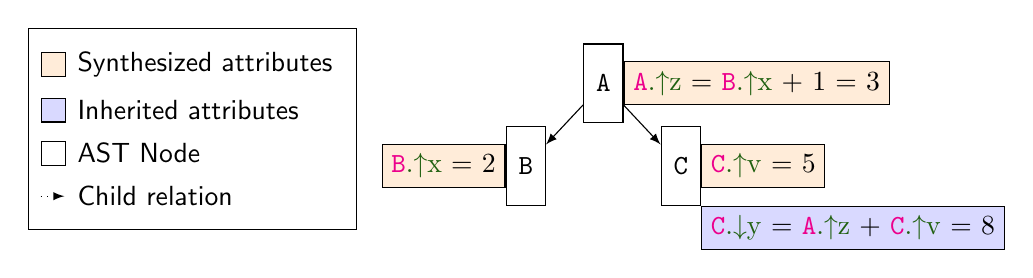
\begin{tikzpicture}[scale=0.7,edge from parent/.style={draw,-latex},sibling distance=8em,
      every node/.style = {align=center,scale=1},
      astnode/.style={shape=rectangle, draw, fill=white, minimum width=5mm,%
      minimum height=10mm},
      synthesized/.style={shape=rectangle, draw, fill=orange!15},
      inherited/.style={shape=rectangle, draw, fill=blue!15}
      ]
    
    \node [astnode,draw] (A) {\code{A}}
      child {node [astnode] (B) {\code{B}}}
      child {node [astnode] (C) {\code{C}}
    }
    ;
    \node [synthesized , draw, right=0pt of A] (AA) {\Asyn{A}{z} = \Asyn{B}{x} + 1 = 3};
    \node [synthesized , draw, left=0pt of B] (BB) {\Asyn{B}{x} = 2};
    \node [synthesized , draw, right=0pt of C] (CC) {\Asyn{C}{v} = 5};
    \node [inherited , draw, below right =0pt of C] (CC) {\Ainh{C}{y} = \Asyn{A}{z} + \Asyn{C}{v} = 8};
    
    \matrix [draw, below right = -50pt and -180pt,inner sep=1ex,cells={nodes={font=\sffamily,anchor=west}}] at (B) {
      \node [synthesized] {}; & \node{Synthesized attributes}; \\
      \node [inherited] {}; & \node{Inherited attributes}; \\
      \node [rectangle,draw] {}; & \node{AST Node}; \\
      \draw[-latex,dotted,color=black](0,0) -- ++ (0.3,0); & \node{Child relation}; \\
    };
    \end{tikzpicture}
    \caption{\label{fig:ragsExample} Graphical representation of the attribute grammar example.}
\end{figure}

Let us consider the following abstract grammar:

    \begin{align*}
        A& ::= B \quad C \\ 
        B& \\
        C&
    \end{align*}

and the following attribute declarations:
    \begin{align*}
        \Asyn{A}{z}& = \Asyn{B}{x} + 1 \\
        \Asyn{B}{x}& = 2 \\
        \Asyn{C}{v}& = 5 \\
        \Ainh{C}{y}& \\
        \Ainhdef{A}{C}{y}& = \Asyn{A}{z} + \Asyn{C}{v} \\
    \end{align*}
The value for the synthesized attribute \Asyn{A}{z} is computed by solving 
the equation systems for the attributes \Asyn{A}{z} and \Asyn{B}{x}:
\begin{align*}
    \Asyn{A}{z} &= \Asyn{B}{x} + 1 \\
    \Asyn{B}{x} &= 2
\end{align*}
leading to \Asyn{A}{z} = 3 and \Asyn{B}{x} = 2.
The value for the inherited attribute \Ainh{C}{y} is defined by the node \astnode{A} for
each child of type \astnode{C}. The value of \Ainh{C}{y} is computed by solving the equation system:
\begin{align*}
    \Ainh{C}{y} &= \Asyn{A}{z} + \Asyn{C}{v} \\
    \Asyn{C}{v} &= 5\\
    \Asyn{A}{z} &= 3
\end{align*}
resulting in \Ainh{C}{y} = 8. Figure~\ref{fig:ragsExample} depicts the described example.


\section{Reference Attribute Grammars}
\label{sec:rag}
Reference Attribute Grammars (RAGs) where introduced in~\cite{DBLP:journals/informaticaSI/Hedin00}
and are an extension of Attribute Grammars to Object-Oriented languages. While attributes in Attribute Grammars
can only refer to terminal values, RAGs allow attributes to refer to non-terminals i.e., node in the AST.
RAGs are well-suited for the analysis of object-oriented languages, since they enable 
the definition of relation between AST nodes. Attributes that refer to 
to AST nodes can declaratively construct relation, i.e., graphs, on the AST.
Examples of the relations that can be constructed using RAGs are:
\begin{itemize}
    \item Name analysis: checks that all names are well-defined and used correctly. A relation between 
    the name and the definition of the name is constructed,
    \item Type analysis: checks that all expressions have a valid type. A relation between the expression
    and its type is constructed,
    \item Graph of a class hierarchy: a graph where nodes are classes and edges are inheritance relations,
    \item Control flow graph: a graph where nodes are statements and/or expressions, and edges are control flow relations, and,
    \item Call graph: a graph where nodes are methods and edges are method calls.
\end{itemize}

\subsection{The JastAdd Metacompiler}
\label{sec:jastadd}
The JastAdd metacompiler~\cite{DBLP:journals/entcs/HedinM01} is a tool for the construction of
Reference Attribute Grammars. The JastAdd metacompiler is a Java-based tool that generates
Java code from a RAG. The generated code can be used to construct an AST and to perform
analysis on the AST.
The JastAdd metacompiler is based on the following components:
\begin{itemize}
    \item The JastAdd language: a language for the definition of RAGs. 
    The JastAdd language allow to specify the abstract grammar of a language, and,
    with a java-like syntax, the attributes of the RAG.
    \item The JastAdd compiler: a compiler that generates Java code from a RAG.
\end{itemize}
In JastAdd, synthesized attributs are defined using the \code{syn} keyword followed
by the type and the name of the attribute. Similarly, inherited attributes are defined
using the \code{inh} keyword. Let us reconsider the example depicted in Figure~\ref{fig:ragsExample}. 
The abstract grammar is defined in a \code{.ast} file with the following syntax:
    \begin{lstlisting}[language=JastAdd]
        A ::= B C;
        B; 
        C;
    \end{lstlisting}
where each line defines a non-terminal, i.e., a node in the AST.
The attributes are defined in a \code{.jrag} file with the following syntax:
    \begin{lstlisting}[language=JastAdd]
        syn int A.z() = B.x() + 1;
        syn int B.x() = 2;
        syn int C.v() = 5;
        inh int C.y();
        eq A.C.y() = A.z() + C.v();
    \end{lstlisting}
The last line is an equation that defines the value of the inherited attribute \Ainh{C}{y} for each child of type \astnode{C}.
\begin{figure}
    \begin{center}
        \begin{tikzpicture}
            \tikzstyle{block} = [rectangle, draw, text centered, minimum height=10em, minimum width=10em]
            \tikzstyle{line} = [draw, -latex]
            \node [block] (A) {
                \begin{lstlisting}[language=JastAdd]
aspect AttrDecl {
  syn int A.x() = 1;
  syn int B.x() = 2;
}
                \end{lstlisting}
            };
            \node [block, right=of A, yshift=5em] (B) {
                \begin{lstlisting}[language=JastAdd]
class A {
    public int x(){
    return 1;
    }
}
                \end{lstlisting}
            };
            \node [block, below=of B] (C) {
                \begin{lstlisting}[language=JastAdd]
class B {
    public int x(){
        return 2;
    }
}
                  \end{lstlisting}
             };
        
             \node (v1) at (-1.3,0) {};
             \node (v2) at (1.8,0) {};
             \node (v3) at (3.1,1.3) {};
             \node (v4) at (6.1,1.3) {};
             \node (v5) at (6.1,2.3) {};
             \node (v6) at (3.1,2.3) {};
             \node (v7) at (1.8,0.3) {};
             \node (v8) at (-1.3,0.3) {};
             \draw[opacity=0.2,fill=blue] (v1.center)--(v2.center)--(v3.center)--(v4.center)--(v5.center)--(v6.center)--(v7.center)--(v8.center)--(v1.center);
        
             \fill [opacity=0.2,blue]
                 (v1) \foreach \i in {2,...,8}{ -- (v\i) } -- cycle;
            
            \node (vv1) at (-1.3,-0.01) {};
            \node (vv2) at (1.8,-0.01) {};
            \node (vv3) at (3.1,-2.3) {};
            \node (vv4) at (6.1,-2.3) {};
            \node (vv5) at (6.1,-3.3) {};
            \node (vv6) at (3.1,-3.3) {};
            \node (vv7) at (1.8,-0.3) {};
            \node (vv8) at (-1.3,-0.3) {};
            \draw[opacity=0.2,fill=red] (vv1.center)--(vv2.center)--(vv3.center)--(vv4.center)--(vv5.center)--(vv6.center)--(vv7.center)--(vv8.center)--(vv1.center);
        
            \fill [opacity=0.2,red]
                (v1) \foreach \i in {2,...,8}{ -- (vv\i) } -- cycle;
        \end{tikzpicture}
    \end{center}
    \caption{\label{fig:interType} Example of intertype declaration.}
\end{figure}


JastAdd supports intertype declarations for the definition of attributes. An intertype declaration
of an attribute is a declaration that is performed into an aspect that, at compile time, 
is inlined in the class specified in the intertype declaration. The example in Figure~\ref{fig:interType}
shows an intertype declaration of an attribute. 
The attribtues \Asyn{A}{x} and \Asyn{B}{x} are defined in the aspect \code{AttrDecl} 
that is inlined in the classes \code{A} and \code{B} respectively.

JastAdd supports not only synthesized and inherited attributes, but also:
\begin{itemize}
    \item \emph{Parametrised Attribute}: the value of the attribute might depend
    not only on the AST node itself, but also on the value of the arguments supplied
    to it. Attributes of this kind are widely used, especially in the definition of 
    type-checking rules.
    \begin{lstlisting}[language=JastAdd]
        syn Type A.compatible(Type t) = this.type() == t;
    \end{lstlisting}
    

    \item \emph{Higher-Order Attribute (HOA)}\footnote{Also known as \emph{Non-Terminal Attributes (NTA)}.}:
    the value of an HOA is a freshly new subtree. Are called \emph{Higher-Order Attributes}
    because are attribute and at the same time a non-terminal, therefore they can be attributed.
    The subtree computed by an HOA behaves like a normal non-terminal, i.e., it can be
    attributed and it can be used in the definition of other attributes. In JastAdd, HOAs
    are defined using the \code{nta} keyword. HOAs are widely used to reify information 
    that are not explicit in the source-code and therefore, not present in the AST.
    For example, when constructing a CFG of a method, is always useful to specify
    a unique entry point and a unique exit point for the method. In JastAdd, this can be
    achived using an HOA:
    \begin{lstlisting}[language=JastAdd]
        syn nta Entry MethodDecl.entry() = new Entry();
        syn nta Exit MethodDecl.exit() = new Exit();
    \end{lstlisting}
    We use the right-arrow symbol to denote HOAs, e.g.,  \Ahoa{MethodDecl}{entry} and \Ahoa{MethodDecl}{exit}.
    \item \emph{Circular Attribute}: an attribute that which definition might depend direclty
    or indirectly on itself. In JastaAdd, circular attributes are expressed using the \code{circular}
    keyword. To guarantee termination, circular attributes are evaluated in a fixed-point
    computation, i.e., the attribute is evaluated until the value of the attribute does not change.
    The requirements, that are not checked by JastAdd, to guarantee termination are:
    \begin{itemize}
        \item All the possible values computed by the attribute must be placed 
        in a lattice of finite height.
        \item The 
    \end{itemize}

    \item \emph{Collection Attribute}: an attribute that returns a collection of values.
\end{itemize}





\subsection{Control-Flow Analysis}
\label{sec:controlflow}
Control-Flow Analysis is a static analysis technique used to determin the control-flow graph (CFG) of a program.
The CFG is a directed graph representing all the possible path that a program can
take during its execution. The CFG of a program is used to perform many static analyses, such as
data-flow analysis, and to perform program transformations, e.g., loop unrolling.


Let us consider the graph $\mathcal{G}=(B,F)$ where $B$ is the set of nodes 
of the graph and $F$ is the set of edges. Each node $b$ of $B$ represents a
basic block of the program. A basic block is a sequence of instructions with one and only one
entry point and exit point. Meaning that there is no jump instruction in the middle of a basic block.
The edges of $F$ represent the possible transitions between basic blocks. Given two
basic blocks $b_1$ and $b_2$, there is an edge \CFGEdge{b_1}{b_2} in $F$ if $b_2$ is an immediate
successor of $b_1$.
\begin{definition}
    Given a basic block $b$, we define the set of successor of $b$ as 
    $$ \text{succ(b)} = \{b_2 \mid \CFGEdge{b}{b_2} \in F\}.$$
\end{definition}
The predecessor relation is defined in a similar way:
\begin{definition}
    Given a basic block $b$, we define the set of predecessor of $b$ as the 
    inverse of the successor relation:
    $$ \text{pred(b)} = \{b_1 \mid \CFGEdge{b_1}{b} \in F\} = \text{succ}^{-1}\text{(b)}.$$
\end{definition}
Among $B$, we can distinguish two special nodes: the entry node $b_{\text{entry}}$ and 
the exit node $b_{\text{exit}}$. The entry node is the node from which the program starts its execution.
The exit node is the node to which the program returns after its execution. The entry node is the only node
with no predecessor, and the exit node is the only node with no successor. More 
formally, we can define the entry node as the unique node $b_{\text{entry}}$ such that
$$ \forall b \in B, \text{pred}(b) \neq \emptyset \Rightarrow b = b_{\text{entry}}.$$
Similarly, we can define the exit node as the unique node $b_{\text{exit}}$ such that
$$ \forall b \in B, \text{succ}(b) \neq \emptyset \Rightarrow b = b_{\text{exit}}.$$
\begin{definition}
    A path in $\mathcal{G}$ is a sequence of basic blocks $b_1, \ldots, b_n$ such that
    $$ \forall i \in \{1, \ldots, n-1\},  b_{i+1} \in \text{succ}(b_i).$$
\end{definition}


Most of the time, the CFG is constructed on top of an intermediate representation
(IR) of the program. The IR is a language that is easier to analyze than the original
source language. The IR is usually a low-level language, such as LLVM IR or Java Bytecode, that are
closer to the machine code than the source language. 
Moreover, since the IR is usually targeted by serveral different langauges, 
it requires less engineering effort to implement a control-flow analysis for the IR than for each
source language.
A less common approach is to construct the CFG on top of the source language.
This method fits well for imperative languages, where the control-flow is 
explicit in the source code. For functional languages, the
control-flow is implicit in the source code, and the CFG is usually constructed
on top of the IR.




\subsection{Control-Flow Analysis Using RAGs}
\label{sec:cfarag}
In this section, we discuss \texttt{JastAddJ-Intraflow}, the first attempt of 
implementing control-flow analysis using RAGs.

Before discussing \texttt{JastAddJ-Intraflow}, we first introduce the 
\bnc\ language, a simple but powerful enough,  imperative language, that we 
will use to illustrate how JastAddJ-Intraflow works.


\subsection{The \bnc\ Language}
\bnc\ is a simple imperative language subset of the C language.
The syntax of \bnc\ is defined by the following abstract syntax:
\begin{lstlisting}[caption={Syntax of the \bnc\ language}]
Program ::= Stmt
Stmt ::= Block | IfStmt | WhileStmt | DeclStmt | AssignStmt
Block ::= Stmt*
IfStmt ::= Cond:Expr Then:Expr Else:Expr
WhileStmt ::= Cond:Expr Body:Expr
DeclStmt ::= Type id Init:Expr
AssignStmt ::= Dest:Expr Source:Expr
Expr ::= id | true | false | Not | And | Or
And ::= Left:Expr Right:Expr
Or ::= Left:Expr Right:Expr
Not ::= Expr
\end{lstlisting}
The starting symbol of the \bnc\ language is the \texttt{Program} non-terminal.
A \texttt{Program} is a list of \texttt{MethodDecl}s. A \texttt{MethodDecl} is a method
declaration, which is composed of a return type, a name, a list of parameters, and a body.
The body of a function is a \texttt{Block}, which is a list of statements. A \texttt{Block}
is a sequence of statements, which can be nested. The statements of SimpliC are
\texttt{IfStmt}, \texttt{WhileStmt}, \texttt{ReturnStmt}, \texttt{ExprStmt}, \texttt{DeclStmt},
and \texttt{AssignStmt}. Reguarding expressions, we decided to include only the most basic
expressions, such as variable reference (\texttt{Id}),  \texttt{Numeral}, boolean values (\texttt{true} and \texttt{false}),
and some binary operators (\texttt{Add}, \texttt{Less} and \texttt{Not}).
For the sake of simplicity, we did not include \texttt{BreakStmt} as the control-flow Analysis
solution is similar to the one of \texttt{ReturnStmt}. 

\subsection{JastAddJ-Intraflow}
\label{sec:jastaddj-intraflow}
The \texttt{JastAddJ-intraflow} (JJI) is the first framework designed for the construction of CFGs
using RAGs. It is not langauge agnostic as it targets the Java language.
JJI is built on top of an earlier version of the ExtendJ Java compiler, called \texttt{JastAddJ}.
The framework is built modularly for each Java version up to Java 7. 
The framework constructs the CFGs and exposes a set of APIs that can be used to 
traverse the CFGs. Listing \ref{lst:jastaddj-intraflow} shows the exposed APIs of JJI.
\begin{lstlisting}[caption={JastAddJ-Intraflow APIs}, label={lst:jastaddj-intraflow}, language=JastAdd]
    public Set<CFGNode> CFGNode.succ();
    public Set<CFGNode> CFGNode.pred();

    public CFGNode CFGNode.entry();
    public CFGNode CFGNode.exit();
\end{lstlisting}
JJI defines the \texttt{CFGNode} interface, which is the base interface for all the nodes in the CFG
and is implemented by all the expressions and statements AST nodes. Each node in the CFG has a set of
successors and a set of predecessors. The entry and exit methods return the reference to entry and exit point of
the enclosing method, respectively.
The possible root of a CFG in JJI is either a method declaration or a constructor declaration. 

The internal APIs of JJI are not intended to be used by the end-users and are used
to build the predecessor and successor sets of each node in the CFG.
The internal API
\begin{lstlisting}[caption={JastAddJ-Intraflow Internal APIs}, label={lst:jastaddj-intraflow-internal}, language=JastAdd]
   Set<CFGNode> CFGNode.following();

   Set<CFGNode> CFGNode.followingTrue();
   Set<CFGNode> CFGNode.followingFalse();
\end{lstlisting}
The \texttt{following} method returns the set of nodes that can be reached after
visiting the current node while the methods \texttt{followingTrue} and \texttt{followingFalse}
are used to model the conditional flow in branches, e.g., \texttt{IfStmt} and \texttt{WhileStmt}, but
also in short-circuiting operators, e.g., \texttt{\&\&} and \texttt{||} in Java.

In terms of RAGs, the framework is defined by the following attributes:
\begin{align*}
    &\Asyn{CFGNode}{succ} = \Asyn{CFGNode}{following} \\
    &\Ainh{CFGNode}{following}  \\
    &\Ainh{CFGNode}{followingTrue}  \\
    &\Ainh{CFGNode}{followingFalse}  \\
    &\Ahoa{CFGNode}{entry} = \text{\emph{fresh }} \astnode{Entry}\\
    &\Ahoa{CFGNode}{exit} = \text{\emph{fresh }} \astnode{Exit}
\end{align*}

The equations for the \texttt{following} attribute are defined based on the context 
of the node. For example, if we consider the \bnc\ language, the \code{Block} node
defines the inherited the attribute \Ainh{Stmt}{following} as follows, where $n$ is the
number of statements in the block:
\begin{align}
    \Ainhindex{Block}{getStmt}{int i}{following} = \begin{cases}
        \Ainh{Block}{following} & \text{if } i=n-1\\
        \{\astnode{Block}.\code{getStmt(i+1)}\} & \text{otherwise}
    \end{cases}
\end{align}
This equation defines the \texttt{following} attribute of the \texttt{Stmt} node 
depending on the position of the statement in the block. If the statement
is the last statement in the block, then the \texttt{following} attribute is
the set of nodes that can be reached after the block. Otherwise, the \texttt{following}
attribute is the set of nodes that can be reached after the next statement in the block.





A limitation of JJI is that allows only the construction of \emph{Parent-first} CFGs.
In a \emph{Parent-first} CFG, the parent node of a node $n$ is always visited before $n$, 
forcing the CFG to be constrained and tight to the AST structure.





\chapter{Dataflow Analysis}
\section{Dataflow Analysis}


% remove the paper number(the LaTeX chapter) from all numberings
\renewcommand{\thesection}{\arabic{section}}
\renewcommand{\thefigure}{\arabic{figure}}
\renewcommand{\thetable}{\arabic{table}}
\renewcommand{\thechapter}{\Roman{chapter}}
\renewcommand{\theequation}{\arabic{equation}}

% include a reference at the footer of reach paper
%\setlength{\chapterdist}{0mm}
\newlength{\apa}
\setlength{\spiff}{0cm}
\renewcommand{\markmargin}{%
	\marginpar{\raggedright \rule{5mm}{0mm}\begin{tikzpicture}
\node[rectangle, fill=black, minimum width=6cm, minimum height=2cm, inner sep=0pt,draw=black](rec){}; \node[left of = rec,node distance=2.7cm,text width=2cm,text centered, font=\sffamily\bfseries\small,rotate=90]{\color{white}{\textsc{Paper \thechapter}}};\end{tikzpicture}\rule{1pt}{\apa}}%
}

\newfloat{paperfoot}{b}{paper}
\newcommand{\paperRemark}[1]{
  \begin{paperfoot}%
  \hrulefill \flushleft \footnotesize #1 \end{paperfoot}
}
%-------------------------------------------------------


\setcounter{chapter}{0}

\renewcommand{\chaptername}{Paper}

\part{Included Papers}


\printbibliography


\end{document}

